\chapter{Desarrollo e implementación}
En este capitulo se desarrolla la solución del problema de validación en la Secretaría de Extensión de la \gls{unam},
en primer instancia se realiza el diseño teórico que se pretende aplicar, su funcionamiento y las relaciones entre las
herramientas y tecnologías en la implementación. 

\section{Tecnologías y Herramientas Seleccionadas}
Las tecnologías y herramientas seleccionadas para el desarrollo de la propuesta son:
\begin{enumerate}
    \item La tesnet llamada Ropsten, esta  Blockchain de prueba es permite publicar los smart contract
    y la emisión de su token de prueba es gratuita, cuenta con pocos nodos pero prácticamente
    la idea es hacer pruebas en esta red, su comportamiento es similar a otra  Blockchain con maquina virtual de ethereum.
    \item Solidity como lenguaje de programación para los contratos inteligentes\cite[]{bragagnolo_smartinspect_2018,dannen_introducing_2017}.
    \item Node JS con su gestor de paquetes para instalar las librerías necesarias.
    \item Web3.js una librería de javascript que permite conectarse a la  Blockchain de una manera mas rápida y abstrayendo la complejidad de la comunicación
    con la Blockchain.\cite[]{dannen_introducing_2017}.
    \item SHA-256 un algoritmo de hash, pero también existen diferentes  librerías de  javascript que permite generar un hash a partir de caracteres.
    \item Vue.js un framework de javascript, para facilitar el desarrollo del front-end, reutilizando partes de otros proyectos open sources.
    \item Para la publicación de los contratos inteligente se usará Remix, es una de las tecnologías ya mencionada y su uso 
    es intuitivo.

\end{enumerate}

Estas tecnologías permitirán crear un sistema para validar si los documentos de la \glsfirst{fce} se pueden 
mantener inmutables en la Blockchain, dando el beneficio a terceros verificar si el contenido de un documento realmente es correcto y no fue alterado. 

\section{Diseño de sistema}\label{s:system_design}
En la sección \ref{ss:basesistema} de la  página \pageref{ss:basesistema} se explica de manera genérica, los datos que se necesitan 
para validar un documento digital en base a los estándares BlockCert y OpenCert.
Para ello se diseña un diagrama de la propuesta del sistema para validar los documentos:  

\begin{figure}[hbt!]
    \centering
    {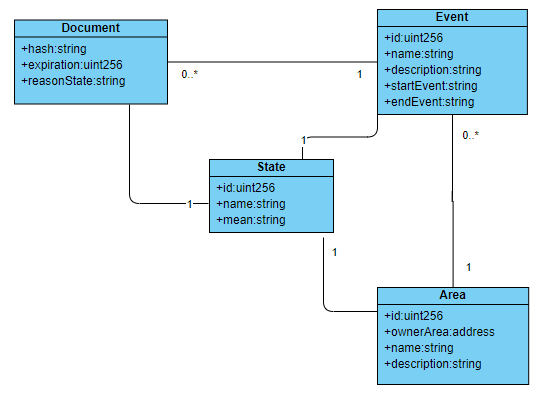
\includegraphics[scale=0.7]{diagrama_clases.png}}
    \caption{Diagrama de domino , elaboración del Autor}
    \label{img:diagrama_clases}
  \end{figure}

  En la figura \ref{img:diagrama_clases} se puede observar la futura  construcción del sistema basándose, 
  en el estándar de blockcerts donde almacenan los hash del documento e información relacionada a ella, y a su vez,
  se agregan información como el evento el cual genera el documento digital,  un área de la organización responsable 
  de emitir esos documentos, y la organización. 
  Estos últimos fueron agregados para poder cubrir algunos aspectos, como en el caso que el documento no refleje la organización que es la responsable de 
  los documentos digitales, también el Área responsable, pero sin revelar datos de personas, por lo tanto el objetivo
  de no incluir  datos sensibles quedan cubiertos. Se analizó
  los requerimientos de la universidad y en conjunto a la entrevista para poder armar la lógica del sistema. También se incluyó administradores o los propietarios (owner) 
  de las áreas, los cuales serían los responsables de almacenar los hashes de los documentos que se generen en los eventos que son parte de sus Áreas,
  cuando se habla de los eventos, se analizó y el evento es totalmente genérico, un evento puede ser una clase, una charla, un congreso o inclusive
  una determinada hora del dia, de esta manera los documentos pueden estar relacionados a los eventos que ocurren.

  El desarrollo del sistema se pretende hacer en un solo smart contract, pueden existir datos que no se reflejen en el diagrama de dominio, 
  ya que la construcción de una aplicación, el almacenamiento y lectura de datos en la  Blockchain es diferente a una 
  aplicación centralizada , por ejemplo los datos almacenados no se consultan mediante lenguaje SQL \cite[]{mayor_Blockchain_2017}, tampoco se puede agregar nuevas
  variables una vez almacenado en la Blockchain, en cambio en una base de datos centralizada si se pueden agregar nuevos atributos \cite[]{dannen_introducing_2017}.

  El Diagrama de la figura \ref{img:diagrama_clases} muestra las relaciones bases del sistema,  como es la lógica y conexión entre los datos.

 

  \subsection{Estructura del smart contract}
  Al definir aproximadamente los datos necesarios para la propuesta del sistema, permite definir 
  la estructura del smart contract, ya que este una vez publicado en la  Blockchain no cambiará, pero no significa
  que se puedan seguir publicando otras versiones, como se va utilizar una  Blockchain de prueba, se pueden realizar todos los intentos necesarios,
  hasta su funcionamiento. 

  La estructura del smart contract será como se refleja en la figura \ref{img:smart_contract_structure}, a continuación se explican cada parte de ella:

  
\begin{figure}[hbt!]
    \centering
    {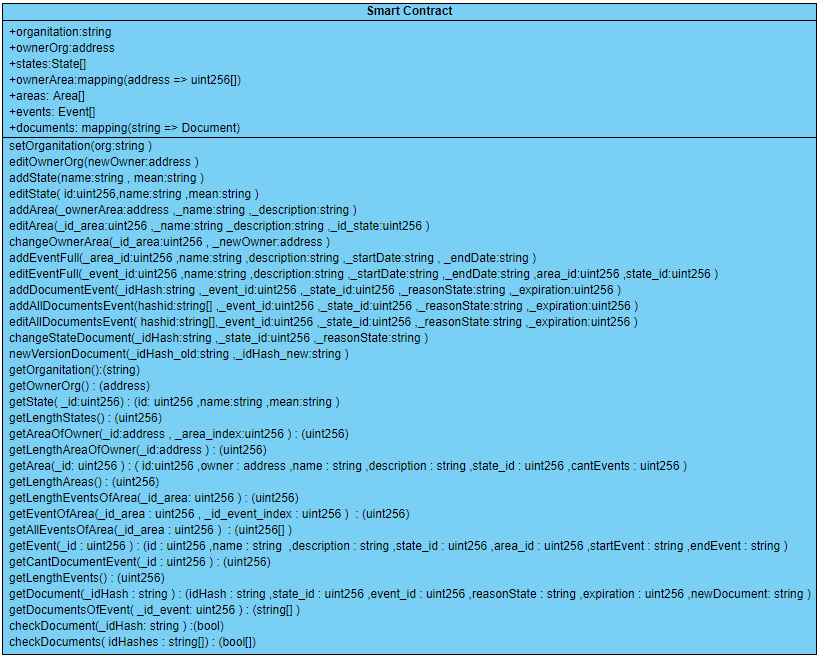
\includegraphics[scale=0.5]{smart_contract_abstract.png}}
    \caption{Smart Contract estructura , elaboración del Autor}
    \label{img:smart_contract_structure}
  \end{figure}
Los atributos que almacenarán los datos necesarios serán:
  \begin{itemize}
    \item organitation:string, se almacenará el nombre de la organización responsable de las áreas, eventos y todos los documento digitales.
    \item ownerOrg:address, la dirección de la cuenta de el único responsable para manejar todos los datos del smart contract.
    \item states: State[], los posibles estados que maneja el sistema, como ser estado revocado, el cual el estándar BlockCert y OpenCert lo usan \cite[]{blockcerts_faq_nodate,opencerts_gestion_nodate}.
    \item ownerArea:mapping(address => uint256[]), son el conjunto de direcciones que están encargadas de manejar una o varias áreas especificas, esto permite 
    estos owner deberian ser agregados por el owner de la organización para evitar que un individuo desconocido tenga el poder de modificar datos.
    \item areas: Area[], el conjunto de áreas de la organización.
    \item events: Event[], los eventos que pueden surgir en un área especifica y encargados de generar los documentos digitales.
    \item documents: mapping(string => Document), 
    \end{itemize}

    La notación que se utilizó para el diagrama \ref{img:smart_contract_structure} para los tipos de datos son de la misma manera
    en la que se definen en solidity,
    como por ejemplo la definición de mapping(string => Document), esto sirve para definir  una variable  que recibe como
    índice un string por ejemplo “A” que referencia un documento almacenado en la Blockchain, el string se creo como índice para 
    que el usuario pueda usar cualquier tipo de algoritmo de hash y el sistema permita almacenar en la  Blockchain sin tomar en cuenta la función hash
    , esta idea es usada por los estándares ya mencionado. 

    Los métodos para realizar cambios en los datos del sistema:
    \begin{itemize}
      \item setOrganitation(org:string), el método permite cambiar el nombre de la organización, este método solo debe ser ejecutado por el propietario de la organización.
      \item editOwnerOrg(newOwner:address ), permite cambiar al único usuario que podrá ejecutar todos los métodos.
      \item addState(name:string , mean:string ), name es el nombre del estado y mean el significado o para que se usaría, el método agrega un nuevo estado que podrá ser usado por las areas, eventos y documentos.
      \item editState( id:uint256,name:string ,mean:string ), edita el nombre y el significado del estado.
      \item addArea(ownerArea:address ,name:string ,description:string ), crea un nuevo estado y pasa por parámetros la dirección del dueño o responsable del área a crear, el nombre y una descripción como dato extra. El único que puede ejecutar este metodo es la direccón que concuerde con la ownerOrg
      \item editArea(id\_area:uint256 ,name:string description:string ,id\_state:uint256 ), el id que representa el área a editar, los datos a modificar como el nombre, la descripción y el estado actual.
      \item changeOwnerArea(id\_area:uint256 , newOwner:address ), permite cambiar el propietario de un área especifica.
      \item addEventFull(area\_id:uint256 ,name:string ,description:string ,startDate:string , endDate:string ), agrega un evento a la  Blockchain relacionándolo, con un área especifica.
      \item editEventFull(event\_id:uint256 ,name:string ,description:string ,startDate:string ,endDate:string ,area\_id:uint256 ,state\_id:uint256 ), edita la mayoría de los atributos de un evento.
      \item addDocumentEvent(idHash:string ,event\_id:uint256 ,state\_id:uint256 ,reasonState:string ,expiration:uint256 ), crea un documento nuevo con relación a un evento particular, y una fecha de vencimiento para el documento digital, la fecha
      es representada por un valor numérico o \gls{TimeStamp}.
      \item addAllDocumentsEvent(hashid:string[] ,event\_id:uint256 ,state\_id:uint256 ,reasonState:string ,expiration:uint256 ), permite almacenar muchos documentos enviando un array de hashes y 
      los atributos iguales que tendran los documentos, por ejemplo todos los documentos serán del mismo evento, tendrán el mismo estado  y fecha de vencimiento.
      \item editAllDocumentsEvent( hashid:string[],event\_id:uint256 ,state\_id:uint256 ,reasonState:string ,expiration:uint256 ), edita todos los documentos que se encuentran en el array de hashes.
      \item changeStateDocument(idHash:string ,state\_id:uint256 ,reasonState:string ), cambia el estado de un solo documento.
      \item newVersionDocument(idHash\_old:string ,idHash\_new:string), se le asigna una nueva versión a un documento antiguo, idHash\_old es el documento antigui y idHash\_new es el hash del nuevo documento,
      esto sirve para mantener versiones de un solo documento. 
    \end{itemize}

    y por último métodos para lectura de los datos, los cuales son:

    \begin{itemize}
      \item getOrganitation():(string), retorna un string que es el nombre de la organziación.
      \item getOwnerOrg() : (address), devuelve la dirección del dueño o propietario, el cual podrá ejecutar todos los métodos.
      \item getState( id:uint256) : (id: uint256 ,name:string ,mean:string ) retorno los atributos del estado que tenga el id pasado por parametro.
      \item getLengthStates() : (uint256), obtiene la cantidad de estados almacenados.
      \item getAreaOfOwner(id:address , area\_index:uint256 ) : (uint256), obtiene el id de un área de un propietario de área.
      \item getLengthAreaOfOwner(id:address ) : (uint256), obtiene la longitud o la cantidad de areas de un propietario de área.
      \item getArea(id: uint256 ) : ( id:uint256 ,owner : address ,name : string ,description : string ,state\_id : uint256 ,cantEvents : uint256 ), obtiene un área a partir de un id.
      \item getLengthAreas() : (uint256), obtiene la cantidad de áreas que hay almacenado en la Blockchain.
      \item getLengthEventsOfArea(id\_area: uint256 ) : (uint256), la cantidad de eventos que están relacionado a un área.
      \item getEventOfArea(id\_area : uint256 , id\_event\_index : uint256 )  : (uint256), obtiene el id un evento relacionado a un área.
      \item getAllEventsOfArea(id\_area : uint256 )  : (uint256[] ), trae todos los id de eventos de un área.
      \item getEvent(id : uint256 ) : (id : uint256 ,name : string  ,description : string ,state\_id : uint256 ,area\_id : uint256 ,startEvent : string ,endEvent : string ), obtiene los atributos de un evento.
      \item getCantDocumentEvent(id: uint256 ) : (uint256),   la cantidad de documentos relacionado a un evento.
      \item getLengthEvents() : (uint256), cantidad de eventos que existen almacenados.
      \item getDocument(idHash : string ) : (idHash : string ,state\_id : uint256 ,event\_id : uint256 ,reasonState : string ,expiration : uint256 ,newDocument: string ), obtiene todo los atributos de un documento a partir de su hash.
      \item getDocumentsOfEvent( id\_event: uint256 ) : (string[]), obtiene todos los hashes de los documentos relacionado a un evento.
      \item checkDocument(idHash: string ) :(bool), devuelve true si el hash del documento esta almcenado en la Blockchain.
      \item checkDocuments( idHashes : string[]) : (bool[]), a partir de un array de hashes de documentos devuelve en el mismo orden true o false dependiendo si existe o no en la Blockchain
      respectivamente.
    \end{itemize}

    \subsection{Roles y permisos}
    En la propuesta de sistema se utilizará un smart contract para el código almacenado en la Blockchain,
    para ello también será necesario definir los responsables de gestionar los datos.
    Se establecen dos niveles, el primero sería un usuario que pueda gestionar todo los datos, como un administrador 
    por ende se debe definir el rol de un usuario o propietario del smart contract, que sea el único que tenga el poder de crear nuevas áreas,
    cambiar en nombre a la organización, editar los datos de las áreas, agregar o quitar responsables de cada área. 
    El otro nivel serían los usuarios encargados de una o muchas  áreas , los cuales tienen la responsabilidad de gestionar los documentos y eventos de un área especifica,
    para ello el administrador o el propietario del smart contract decide quienes son los operarios o encargados de crear los documentos digitales y almacenarlos en la  Blockchain mediante
    su hash.
    Esto es importante para evitar que usuarios externos a la organización controlen los documentos emitidos por la entidad. Para ello se crean los roles o niveles de seguridad.
    En resumen se definen dos niveles nivel uno de administrador que es el encargado y responsable de todo los datos almacenados, por otro lado un nivel de encargados de  áreas.
  \subsubsection{Estructura de permisos}
  Los atributos del smart contract, todos los usuarios tendrán acceso a leer sus datos, por eso se partía del principio de evitar almacenar datos sensibles relacionados
  a los dueños de los documentos, mientras que los datos de la organización son públicos y pueden ser almacenados. 
  En esta sección se definirán que comportamiento tendrán los roles y que permisos según los niveles de usuarios. Analizando los datos sobre los métodos y las necesidades 
  a satisfacer, se parte de tres niveles: 
  \begin{enumerate}
    \item Nivel público, el usuario podrá consultar datos almacenados, como verificar si un documento existe en la Blockchain.
    \item Nivel de propietario de área, son los encargados de almacenar y crear los eventos relacionado a sus áreas, también de gestionar los documentos digitales, cambiando sus estados,
    agregando nuevas versiones.
    \item Nivel de propietario del smart contract, es la única dirección que tiene permiso de ejecutar todos los métodos, puede cambiar el nombre de la organización,
    asignar nuevos propietarios de áreas, crear áreas, y hacer lo mismo que los demás niveles. 
  \end{enumerate}
  
    
    



\section{Desarrollo Smart Contract}

\subsection{Metamask instlación}

Como primer paso hay que instalar el plugin de metamask de su  página web oficial\footnote{\href{https://metamask.io/download.html}{Metamask Página Web }} en el navegador que se usará de prueba en este proceso el navegador es  Google Chrome, 
esto se puede observar en la figura \ref{img:metamask_install}.
\begin{figure}[hbt!]
  \centering
  {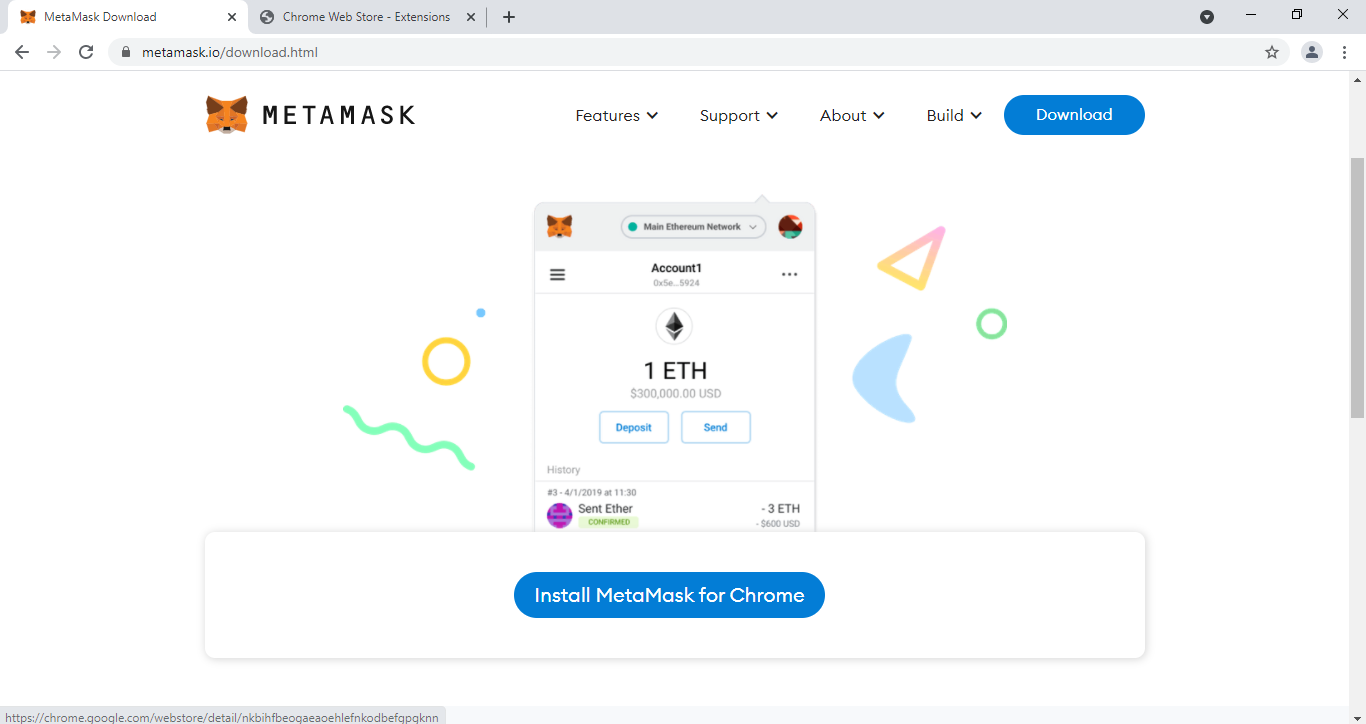
\includegraphics[scale=0.4]{metamask_install.png}}
  \caption{Página para descargar Metamask,  Fuente: captura de pantalla. }
  \label{img:metamask_install}
\end{figure}

Se agrega el plugin al navegador como en la figura \ref{img:metamask_add}, luego
se abrirá una nueva pestaña o en caso que no aparezca deberá buscar metamask en sus extensiones del navegador 
para darle click donde este le redirigirá a una nueva pestaña para crear o importar su wallet.
Los pasos son darle click a Get Stated visto en la figura \ref{img:metamask_getstarted}.



\begin{figure}[hbt!]
  \centering
  {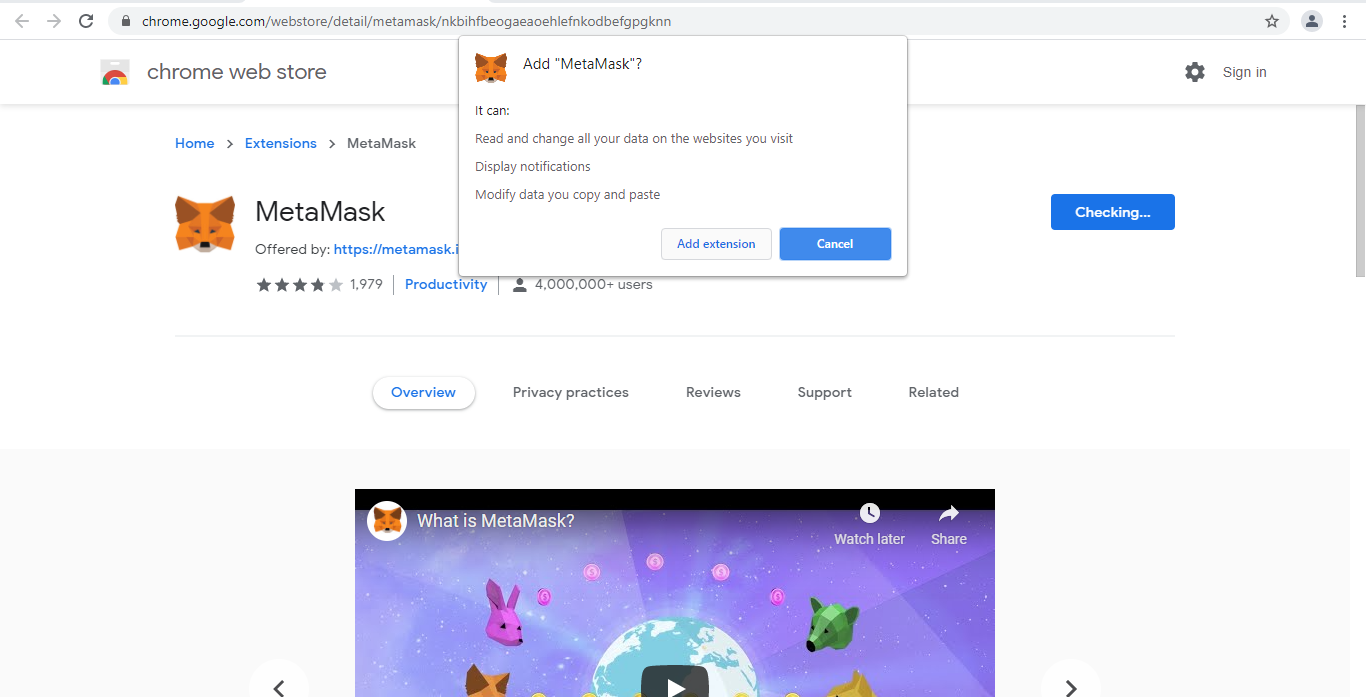
\includegraphics[scale=0.4]{metamask_addplugin.png}}
  \caption{Agregando el plugin , Fuente: captura de pantalla. }
  \label{img:metamask_add}
\end{figure}

\begin{figure}[hbt!]
  \centering
  {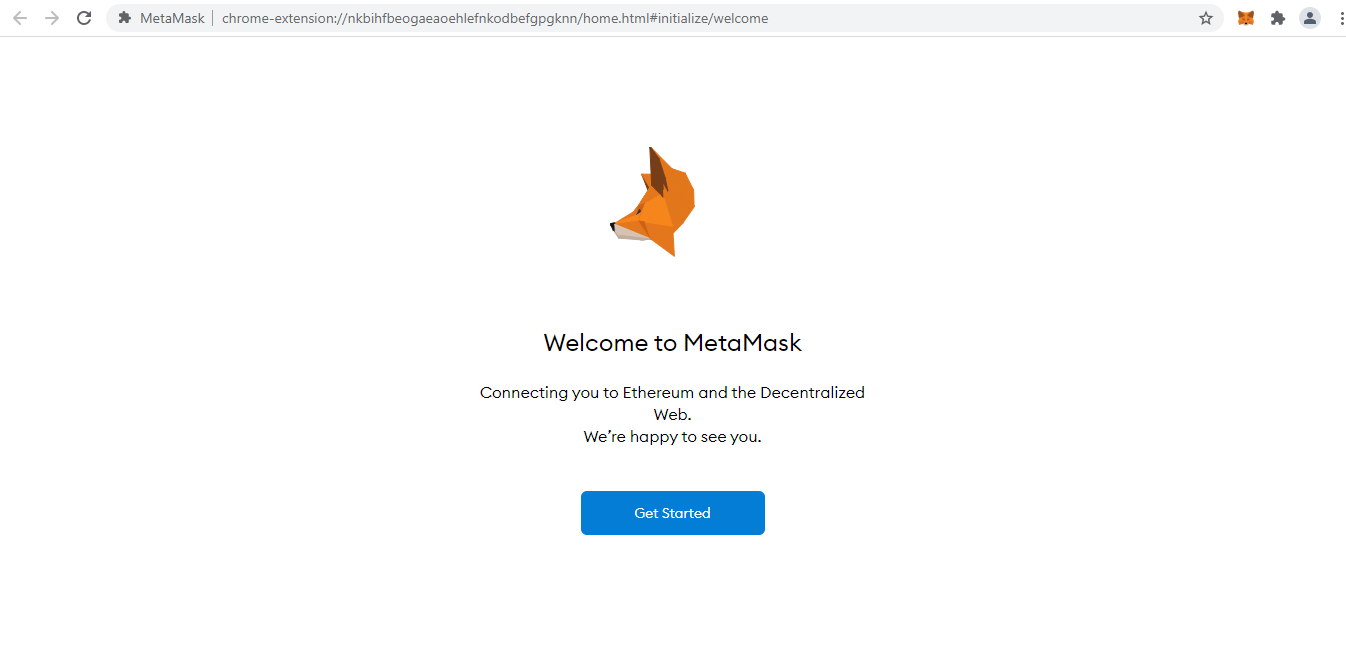
\includegraphics[scale=0.4]{metamask_getstarted.png}}
  \caption{Inicio para crear o importar una wallet, Fuente: captura de pantalla. }
  \label{img:metamask_getstarted}
\end{figure}

Como siguiente paso hay que crear una wallet , esto es importante para poder interactuar con el sistema
específicamente con los smart contract. Leer los términos y condiciones si están de acuerdo aceptarlos,
el siguiente paso es crear una contraseña, esta sirve para acceder a metamask en el computador local, sirve para 
que otro usuario no pueda acceder si no conoce la contraseña y agregar un nivel mas de seguridad, ya que una vez 
adentro se pueden realizar cualquier tipo de operaciones.

\begin{figure}[hbt!]
  \centering
  {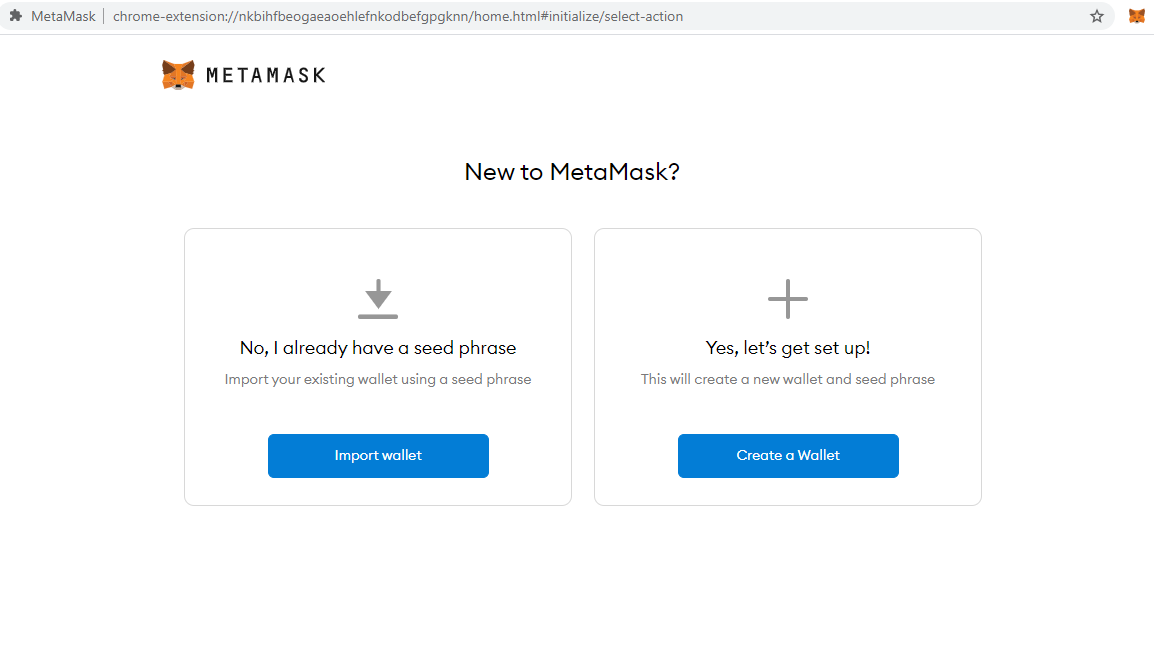
\includegraphics[scale=0.4]{metamask_create.png}}
  \caption{Menu crear wallet, Fuente: captura de pantalla. }
  \label{img:metamask_create}
\end{figure}

\begin{figure}[hbt!]
  \centering
  {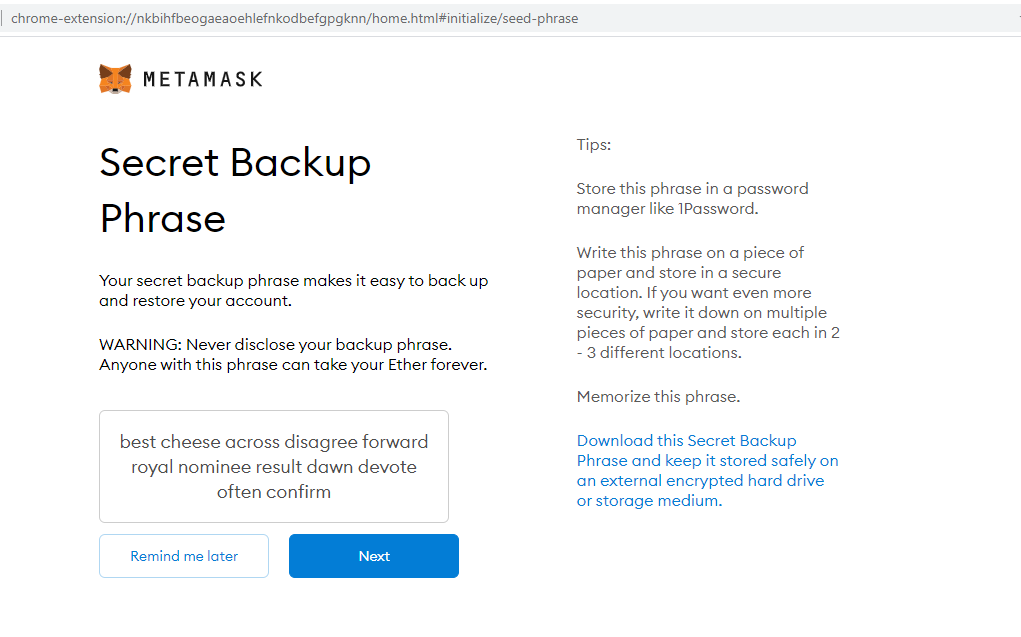
\includegraphics[scale=0.4]{metamask_semilla.png}}
  \caption{Frases semillas ¡NUNCA REVELARLAS!, Fuente: captura de pantalla. }
  \label{img:metamask_semilla}
\end{figure}

Un vez ingresada la contraseña se mostrara su frase semilla de su wallet, como se observa en la figura \ref{img:metamask_semilla},
la frase semilla se muestra de modo didáctico, pero uno NUNCA se repite NUNCA debe compartirlo, porque 
el usuario que conoce su frase semilla podrá abrir la wallet desde otro metamask y hacer lo que desee con ella,
la única manera que otro usuario no pueda intervenir o manejar su wallet es que no conozca su frase semilla, 
por ello es muy importante guardarla en un sitio que solo la personas dueña de la frase semilla conozca,  
a partir de esta frase se genera su llave privada.
La frase semilla generada para esta investigación será rechazada y se usarán otras.
Finalizado la creación de la wallet, se podrá fijar en la parte derecha como se muestra en la figura \ref{img:metamask_new}
\begin{figure}[hbt!]
  \centering
  {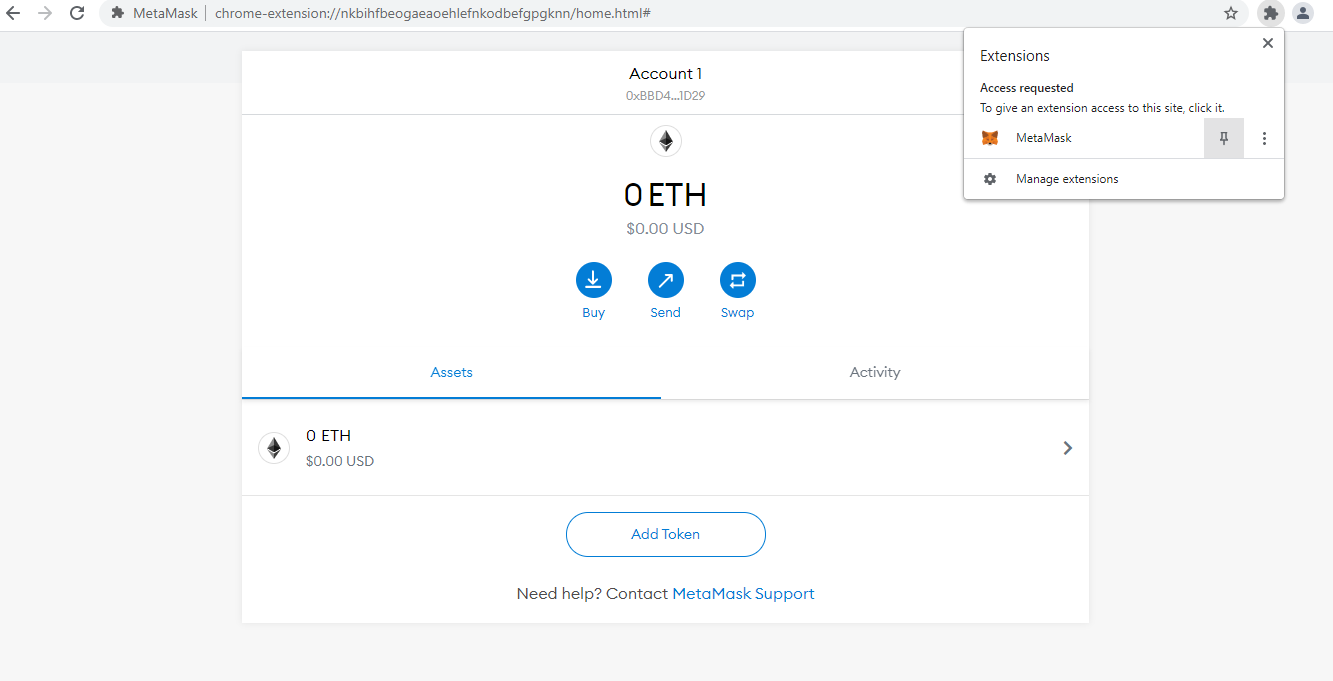
\includegraphics[scale=0.4]{metamask_new.png}}
  \caption{Creación de la wallet finalizada, Fuente: captura de pantalla. }
  \label{img:metamask_new}
\end{figure}


\subsection{Desarrollo del smart contract}
Se utilizó Remix para  la edición del código fuente escrito en solidity para la propuesta de sistema, este programa 
permite compilar el código para probarlo de manera local y también es una herramienta para publicarlo de manera online en otras Blockchain.
En este caso se público en Ropsten.

El código para smart contract se desarrollo siguiendo las definiciones de la sección \ref{s:system_design}, se encuentra en el anexo \ref{as:codigo_smart_contract}
En él se definieron los métodos ya mencionados y se agregaron reglas para que métodos en particulares puedan ser ejecutados solo por el propietario del smart contract y otros 
solo para los propietarios de las áreas.

El código desarrollado, cumple con los principios descriptos en otras secciones, 
y sigue algunas pautas de los estándares de certificados ya mencionados como BlockCerts y OpenCerts.
algunas pautas son, almacenar información del emisor, almacenar el hash del documento, no relacionar datos
personales del propietario del documento digital.

 

\begin{figure}[hbt!]
  \centering
  {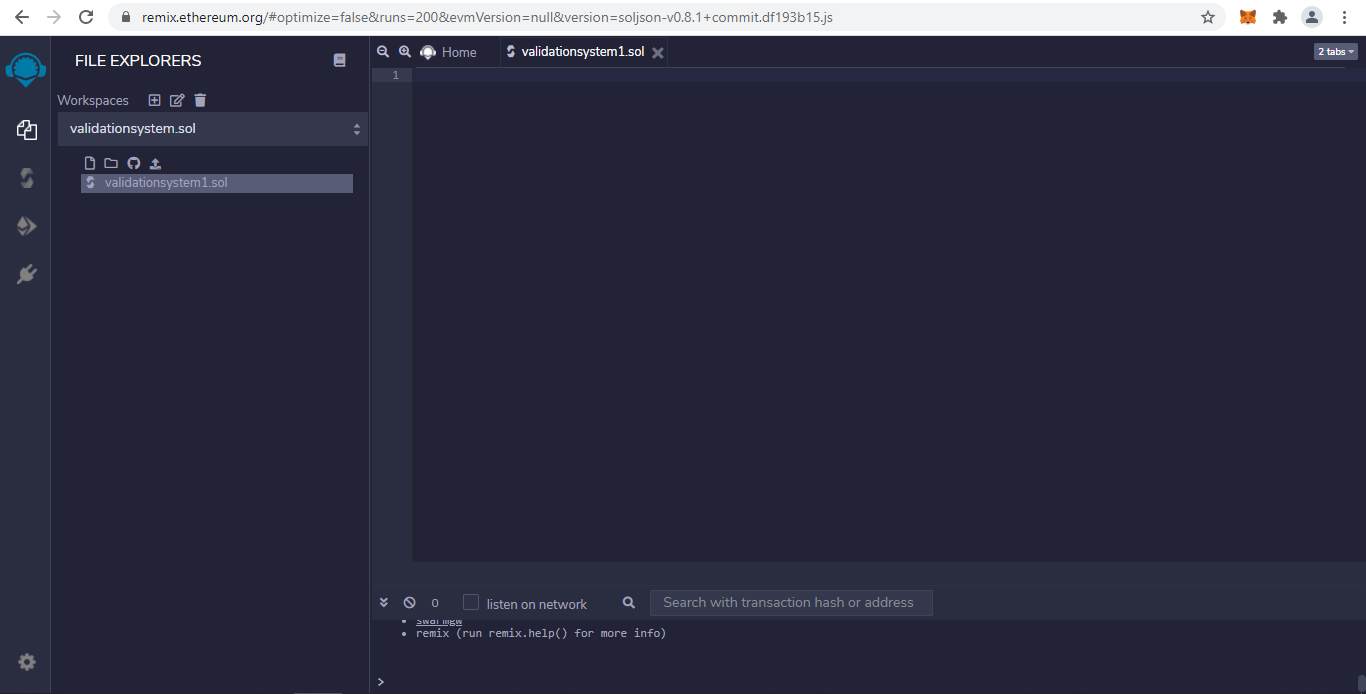
\includegraphics[scale=0.4]{validationSystem.png}}
  \caption{Creando el smart contract con extensión “.sol”, Fuente: captura de pantalla. }
  \label{img:valdationSystem}
\end{figure}

Luego se desarrolla el código dentro del archivo “validationsystem.sol”, que tiene toda la lógica
del sistema con los comportamientos que se pueden realizar.
Una vez esta el código finalizado, hay que compilarlo, en la figura   \ref{img:smart_contract_compile}
muestra como resulta una compilación exitosa.
\begin{figure}[hbt!]
  \centering
  {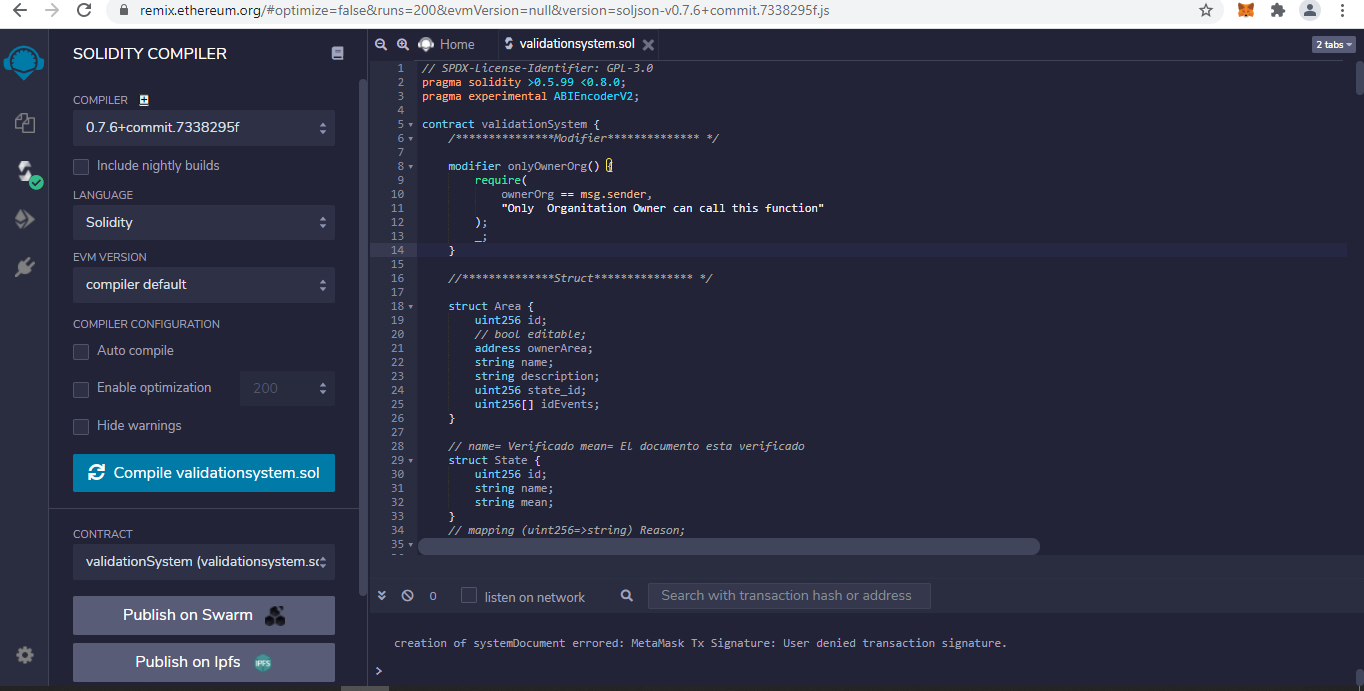
\includegraphics[scale=0.4]{smart_contract_compile.png}}
  \caption{Vista como compilar el contrato, Fuente: captura de pantalla. }
  \label{img:smart_contract_compile}
\end{figure}


Por otra parte es un requisito públicar el smart contract en alguna Blockchain, como se ha mencionado Ropsten
es la seleccionada, para ello hay que abrir metamask y seleccionar la red de Ropsten (Figura \ref{img:ropsten_selected}).
Luego es necesario conseguir la criptomoneda nativa de la Blockchain, como es una red de prueba se consigue de manera gratuita
ingresando a un sitio web de \gls{faucet} que pertmite obtenerlo como por ejemplo uno proporcionado por Metamask \footnote{\url{https://faucet.metamask.io/}} u otro 
proporcionado por Ropsten \footnote{\url{https://faucet.ropsten.be/}}  
\begin{figure}[H]
  \centering
  {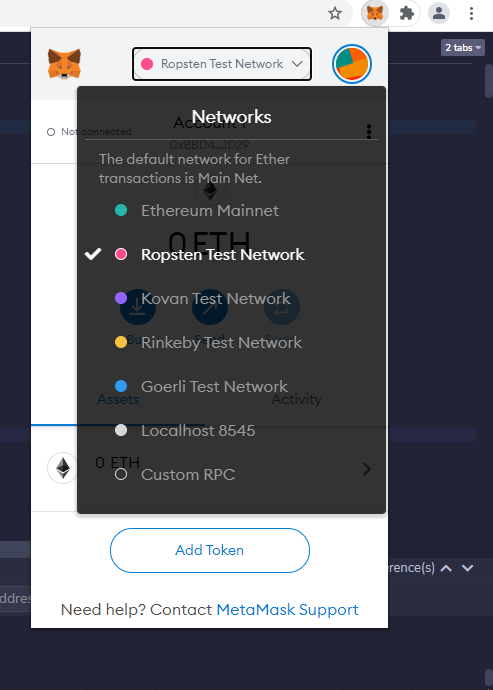
\includegraphics[scale=0.7]{Ropsten_seleteced.png}}
  \caption{Seleccionando la Red de Ropsten, Fuente: captura de pantalla. }
  \label{img:ropsten_selected}
\end{figure}

En este caso se utilizó el sitio web de la figura \ref{img:faucet_metamask} que dándole click al botón verde,
suma 1 ETH a su cuenta.
\begin{figure}[H]
  \centering
  {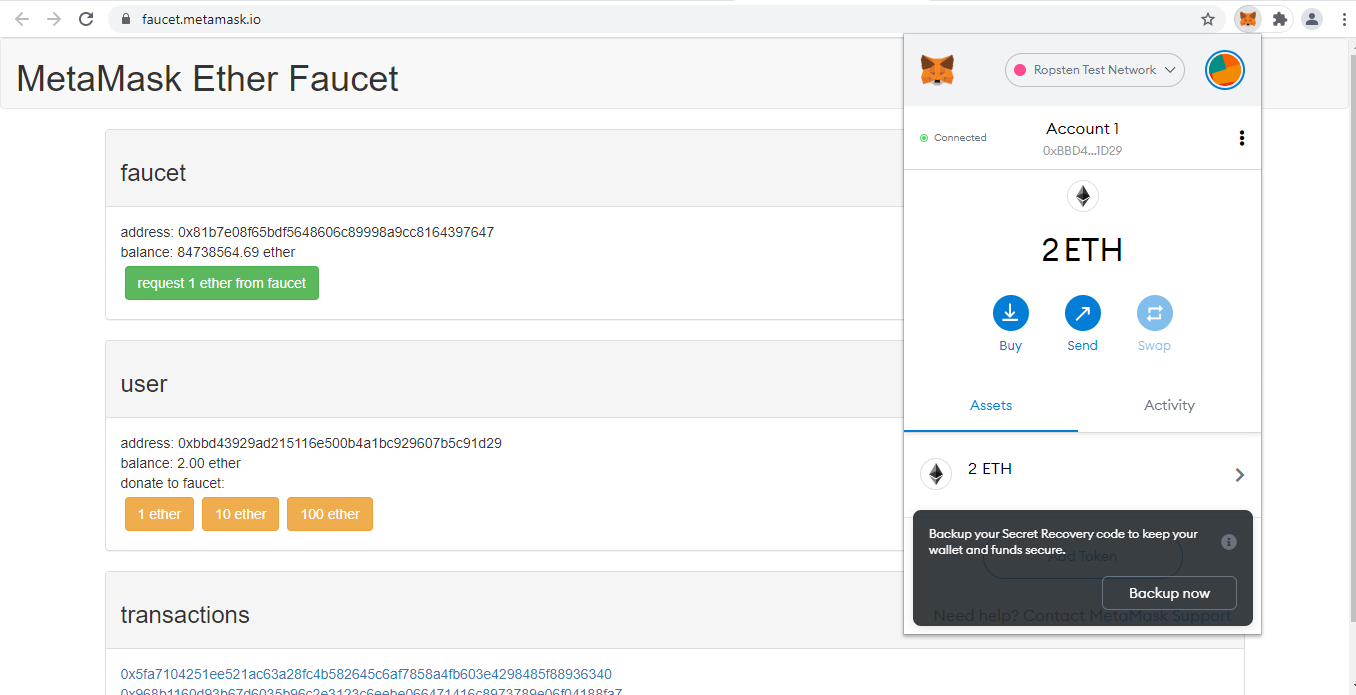
\includegraphics[scale=0.4]{FaucetMetamask.png}}
  \caption{Grifo de MetaMask, Fuente: captura de pantalla. }
  \label{img:faucet_metamask}
\end{figure}

A partir de ahora se cuentan con todas las condiciones para públicar el código en la  Blockchain de Ropsten,
para ello en el menu izquierdo de Remix  seleccionar la opción de  deploy , dentro de ella en la opción de “enviroment”  seleccionar  “inject web3”, 
esto abrirá metamask requiriendo conectar la wallet con el sistema de Remix. Luego dar click al botón de color naranja (deploy) que se observa en la Figura \ref{img:remix_compile}

\begin{figure}[H]
  \centering
  {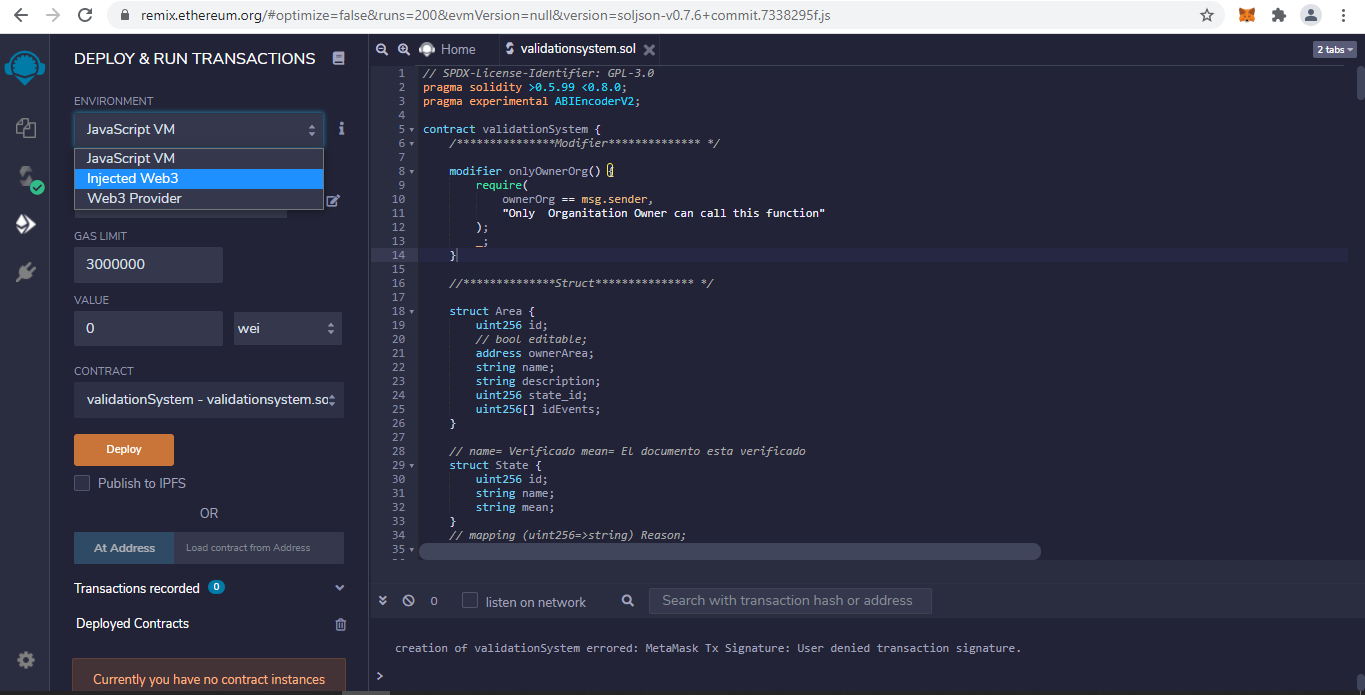
\includegraphics[scale=0.4]{remix_compile.png}}
  \caption{Menu deploy Remix, Fuente: captura de pantalla. }
  \label{img:remix_compile}
\end{figure}

\begin{figure}[H]
  \centering
  {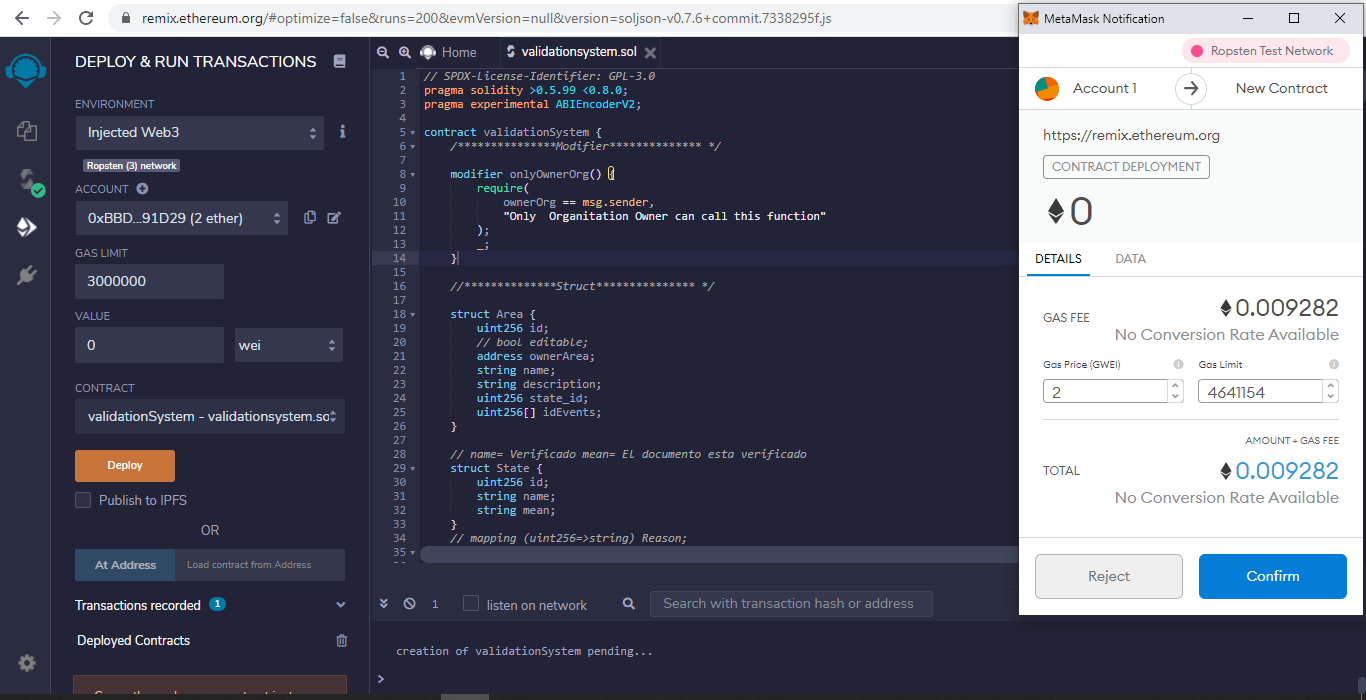
\includegraphics[scale=0.4]{remix_deploy.png}}
  \caption{Deploy Contrato Inteligente, Fuente: captura de pantalla. }
  \label{img:remix_deploy}
\end{figure}

Se abrirá una ventana de metamask (Figura \ref{img:remix_deploy}), que pedirá la confirmación para gastar una cantidad de ETH, que es la criptomoneda
que se ha obtenido mediata el grifo o faucet, la cual se utiliza para pagar las transacciones en la Blockchain.
Se confirma la transacción, y quedará en pendientes hasta ejecutarse, una vez finalizada el smart contract estará en la  Blockchain lista para
usarla.
En la figura \ref{img:metodos_contract_deploy} se muestran los metodos del contrato que se pueden ejecutar en la Blockchain, la interfaz
Remix también sirve para llamar a los diferentes métodos creados.
\begin{figure}[hbt!]
  \centering
  {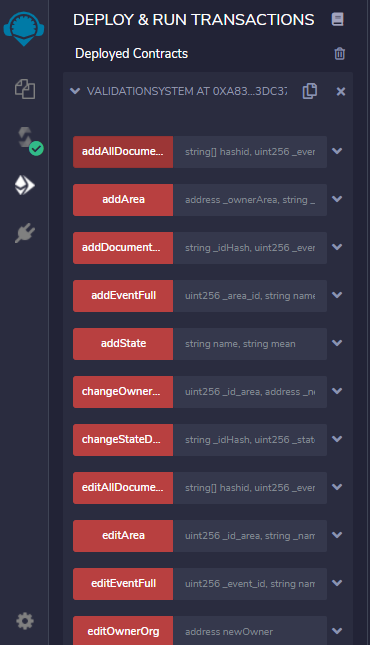
\includegraphics[scale=0.7]{Metodos_contract_deploy.png}}
  \caption{Contrato en la  Blockchain de Ropsten, Fuente: captura de pantalla. }
  \label{img:metodos_contract_deploy}
\end{figure}


\section{Desarrollo de la interfaz de usuario}
El desarrollo se realizará con el sistema operativo Windows 10 Home.
Como primer paso se requiere instalar NODE JS desde su sitio oficial \footnote{\url{https://nodejs.org/en/}},
también se utilizará Visual Studio Code como editor de texto \footnote{\url{https://code.visualstudio.com/}}.

Otro punto es instalar  VUE JS CLI para facilitar la instalación de todos los paquetes y tener una estructura mas organizada \cite[]{vue_cli_overview_2019},
para ello previamente se requiere instalar  NODE JS, en cmd o la consola de comandos del Visual 
Studio Code ejecuta el comando “npm install -g @vue/cli”, para instalarlo de manera global,
en la figura \ref{img:INSTALL_VUE_CLI} se realiza utilizando Visual Studio Code.

\begin{figure}[hbt!]
  \centering
  {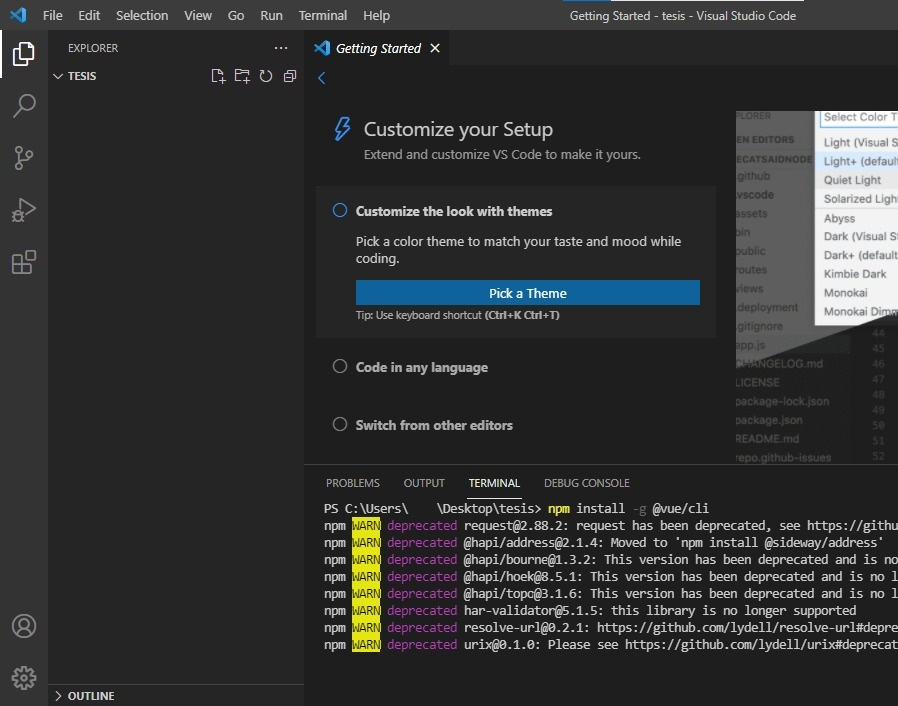
\includegraphics[scale=0.7]{INSTALL_VUE_CLI.jpeg}}
  \caption{Comando para instalar VUE CLI, Fuente: captura de pantalla. }
  \label{img:INSTALL_VUE_CLI}
\end{figure}

Luego en la consola de comando hay que ubicarse en el directorio que se desea instalar el proyecto, una vez hecho esto ejecutar el comando 
“vue create nombre\_proyecto”, en este caso se uso “ vue create validation\_system” esto abrirá unas opciones de configuraciones en consola, 
para el proyecto se utiliza router, vuex, babel; seleccionado estos items continuar con la instalación, en la figura \ref{img:vue_config} se muestra
las opciones necesarias para la creación del proyecto.

\begin{figure}[hbt!]
  \centering
  {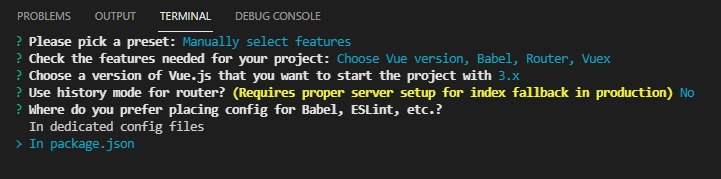
\includegraphics[scale=0.6]{VUE_Config.jpeg}}
  \caption{Configuración de proyecto, Fuente: captura de pantalla. }
  \label{img:vue_config}
\end{figure}

Como siguiente paso ingresar dentro del directorio del proyecto creado en el cual se usarán dos librerías ya mencionadas como web3 \cite[]{web3js_web3js_2016}, sha256 \cite[]{satoh_asic-hardware-focused_2007}, también se usará un componente
que facilita la creación y carga de los select múltiples \footnote{\url{https://github.com/vueform/multiselect}} utilizando VUE, la instalación de estos se realiza con los comandos mostrados en la figura \ref{img:libreria}

\begin{figure}[hbt!]
  \centering
  {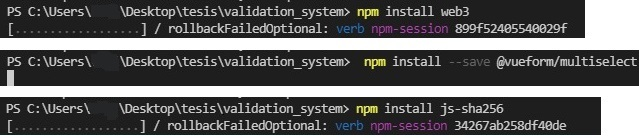
\includegraphics[scale=0.7]{librerias.jpeg}}
  \caption{Instalación de librerías y componente, Fuente: captura de pantalla. }
  \label{img:libreria}
\end{figure}

A partir de este punto empieza el desarrollo de la interfaz gráfica con las librerías y herramientas instaladas.

\subsection{Desarrollando vista del sistema}
Inicialmente, teniendo la carpeta del proyecto generada se crean unos archivos extras, en este caso dentro de la ruta del proyecto “nombre\_proyecto/src/” se crea una carpeta con el nombre \/app donde
se almacenarán archivos que permitirán conectar con la Blockchain,

\begin{figure}[H]
  \centering
  {\includegraphics[scale=0.7]{ruta_archivo_Blockchain.png}}
  \caption{Archivos para conexión con la Blockchain, Fuente: captura de pantalla. }
  \label{img:ruta_archivo_Blockchain}
\end{figure}
el archivo abi.js define todos los métodos o funciones que se pueden usar en el smart contract creado, para eso 
habría que ir a Remix, compilar nuevamente el código del smart contract y copiar el \gls{abi} creado. Por ejemplo 
en la figura \ref{img:abi_copy} se resalta con un circulo rojo, el botón para copiar el ABI, este código se pega 
dentro de la carpeta abi.js, el \gls{abi} es utilizada para  las llamadas a los métodos.

\begin{figure}[H]
  \centering
  {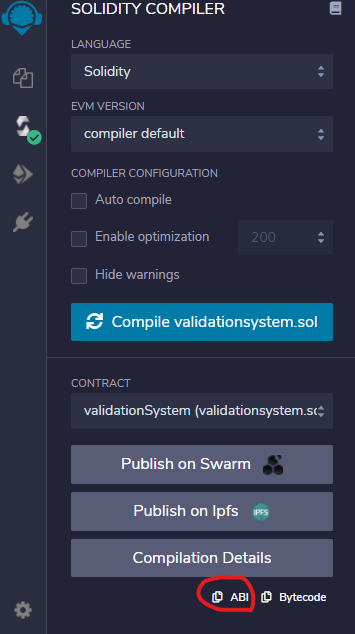
\includegraphics[scale=0.7]{ABI_Copy.png}}
  \caption{Copiar el ABI del código, Fuente: captura de pantalla. }
  \label{img:abi_copy}
\end{figure}

Posteriormente se crean una serie de archivos como app.js, document.js, parameters.js que contendrán la lógica para conectar la vista frontal con la Blockchain.
El último archivo parameters.js almacena la dirección del smart contract, la dirección se crea en el momento que se publicó el código con Remix ,
la dirección generada fue “\textbf{0x7006882779C21D8246 C82989F813237f78A781b1}”.


Las vistas desarrolladas  con VUE JS:
\begin{enumerate}
  \item Gestión de Área: permite crear  Áreas, asignar un propietario mediante una dirección o clave pública, un nombre, descripción,
  a partir de él se pueden crear eventos.

  \begin{figure}[H]
    \centering
    {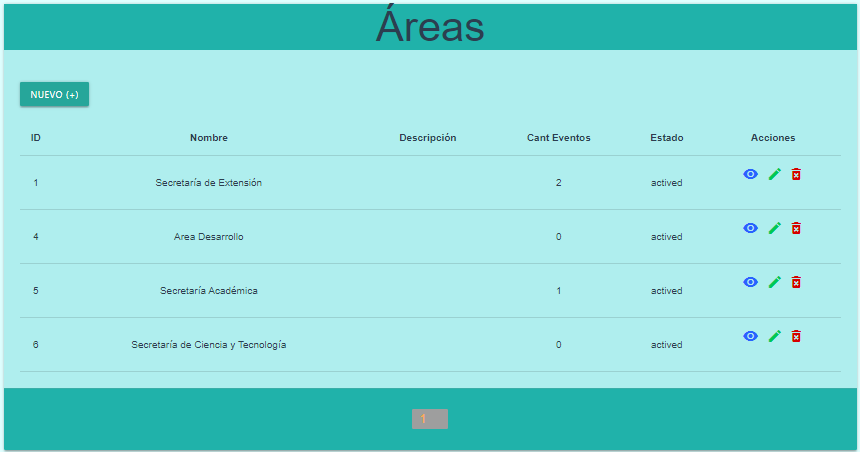
\includegraphics[scale=0.7]{Front_Area.png}}
    \caption{Vista de Áreas, Fuente: captura de pantalla. }
    \label{img:front_area}
  \end{figure}

  \item Gestión de Evento: se crean los Eventos encargados de generar los documentos, los datos para crear un evento son el nombre, 
  área relacionada, descripción, fecha de cuando inicio el evento, fecha cuando finaliza el evento y un estado. 
  La fechas sirven para saber en que periodo se crearon los documentos, ya que cada documento esta relacionado  a un evento.
  \begin{figure}[H]
    \centering
    {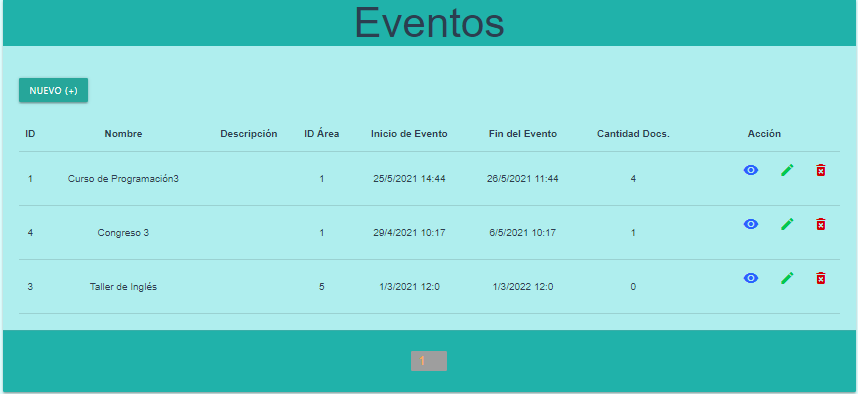
\includegraphics[scale=0.7]{Front_event.png}}
    \caption{Vista de Eventos,  Fuente: captura de pantalla. }
    \label{img:front_event}
  \end{figure}     
  
  \item Gestión de Documentos: Se verifican o validan los documentos, si el usuario tiene el rol para crear documentos 
  también se utiliza como carga del mismo, si no tiene un rol solamente puede verificar si el documento fue registrado por la organización. 
  Un usuario propietario del área ve como se muestra en la figura \ref{img:front_document_owner}  
  \begin{figure}[H]
    \centering
    {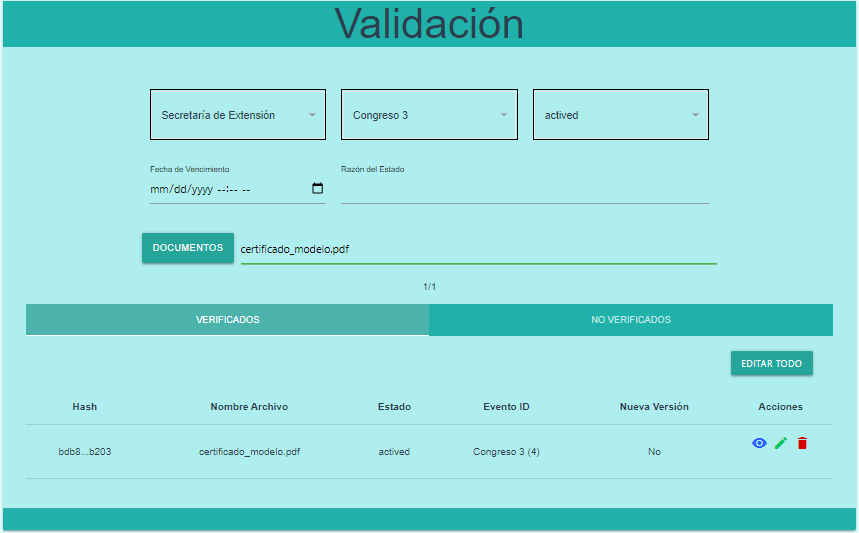
\includegraphics[scale=0.7]{Front_document_owner.png}}
    \caption{Vista de Documentos como propietario,  Fuente: captura de pantalla. }
    \label{img:front_document_owner}
  \end{figure}
  y en el caso de una dirección pública que 
  no está registrado como propietario de un área o de la organización visualiza los documentos como en la figura \ref{img:front_document_public}
  \begin{figure}[H]
    \centering
    {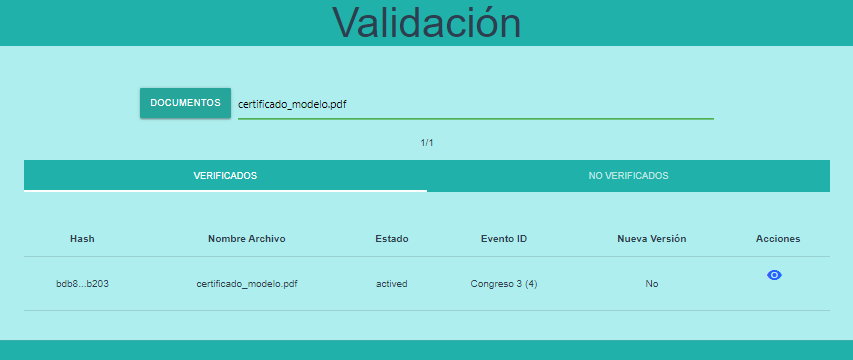
\includegraphics[scale=0.7]{front_document_public.png}}
    \caption{Vista de Documentos como usuario público,  Fuente: captura de pantalla. }
    \label{img:front_document_public}
  \end{figure}

  \item Gestión de Organización: Mantiene los datos de la Organización, permite cambiar el nombre, cargar nuevos estados y cambiar al propietario de la organización, que 
  en este caso es el usuario que tiene permitido todas las acciones creadas.
  Los estados cargados por defecto son “ deleted ”, “ actived ”, “ expired ” y no pueden ser eliminados en el sistemas  ni modificados excepto “ expired ” 

  \begin{figure}[H]
    \centering
    {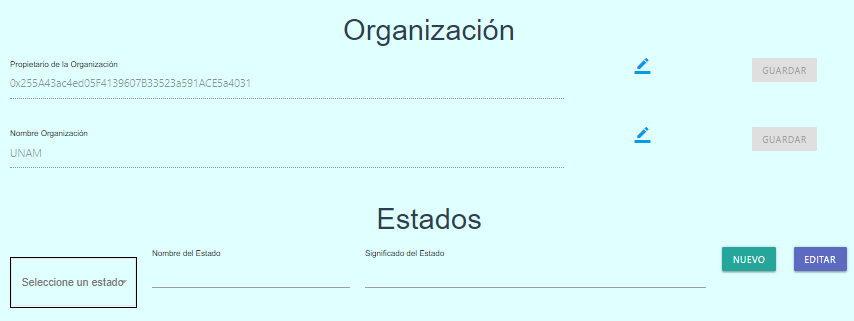
\includegraphics[scale=0.4]{front_org.png}}
    \caption{Vista de Organización,  Fuente: captura de pantalla. }
    \label{img:front_org}
  \end{figure}
\end{enumerate}

El código completo del front end se encuentra en el repositorio de git \footnote{\url{https://github.com/agustinbritez/Sistema_Validacion.git}} 

\section{Pruebas del Sistema}
La prueba inicia cargando los datos base como el nombre de la Organización, las áreas que responsables de los eventos que emitirán los documentos.
Partiendo de un smart contract desplegado como se mostrá en otras secciones, el administrador o propietario de la organización concuerda con la dirección encargada 
de publicar el contrato inteligente, pero este puede ser cambiado por otro.
\subsection{Preparando el sistema}

Se cambia el nombre de la organización a “ Universidad Nacional de Misiones Facultad de Ciencias Económicas ”, esto sirve para identificar el nombre de la organización, se 
crean estados nuevos como “ en espera ”, “ on hold ” \ref{img:cambio_org}.
Se crean las Áreas de la Organización, es este caso “ Secretaría de Extensión ” , con el propietario del área con dirección  “ 0x255A43ac4ed05F41396 07B33523a591ACE5a4031”
y el estado “ actived ” \ref{img:nuva_area}.
\begin{figure}[H]
  \centering
  {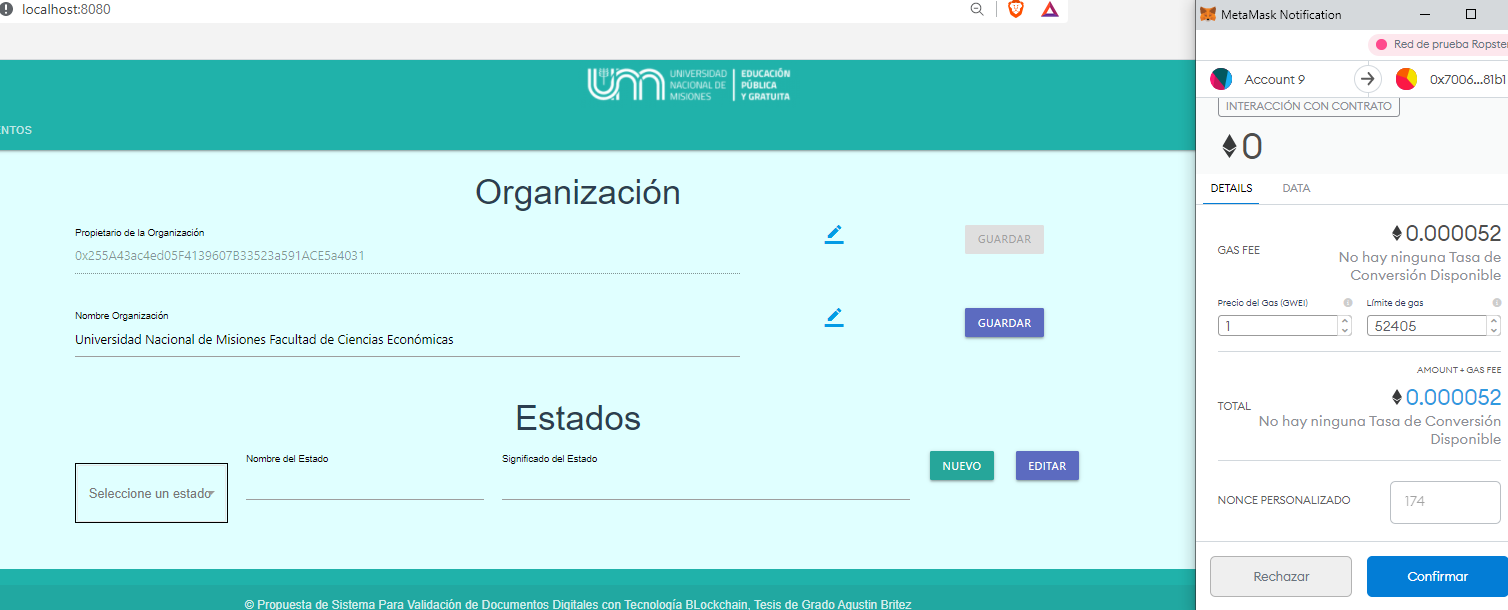
\includegraphics[scale=0.4]{cambio_organizacion.png}}
  \caption{Cambio de nombre de la organización,  Fuente: captura de pantalla. }
  \label{img:cambio_org}
\end{figure}

\begin{figure}[H]
  \centering
  {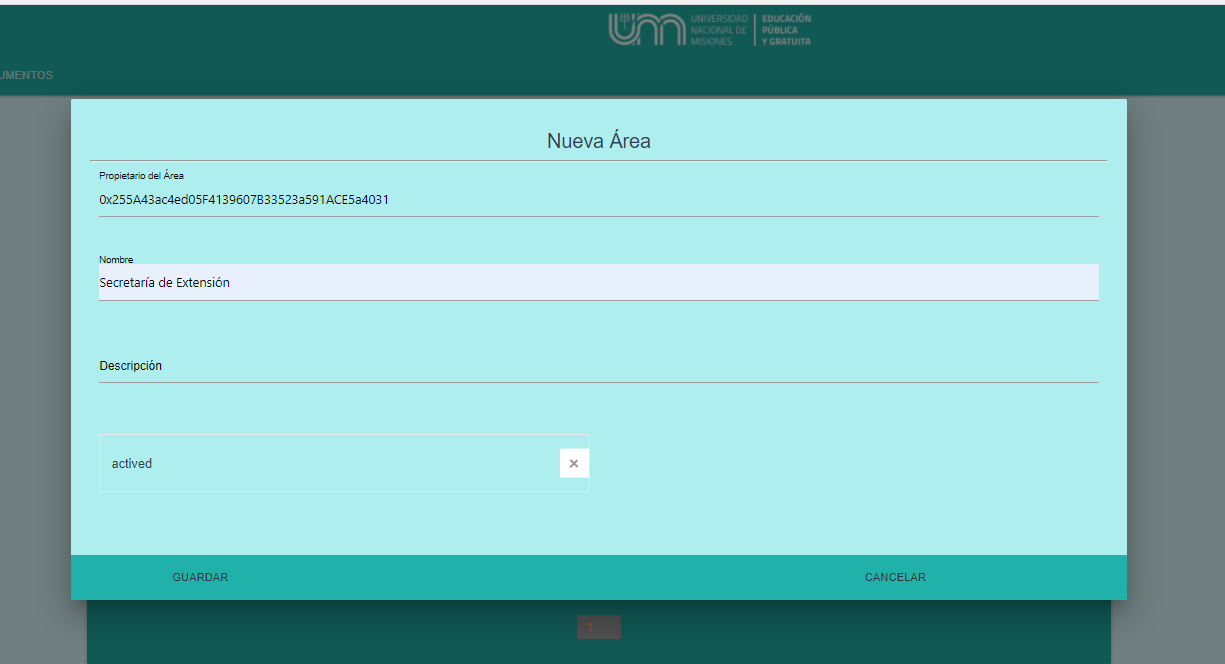
\includegraphics[scale=0.4]{nueva_area.png}}
  \caption{Creación de nueva área en el sistema,  Fuente: captura de pantalla. }
  \label{img:nuva_area}
\end{figure}
Se requiere un evento el cual genera los documentos, por ende se crea uno con el nombre de “ Curso de Economía Actual ” , que se relaciona al área recién mencionada que es 
“ Secretaría de Extensión ” con una fecha de inicio del evento el “ 18/05/2021 08:00hs” y fecha de finalización “ 20/05/2021 08:00hs ”.
\begin{figure}[H]
  \centering
  {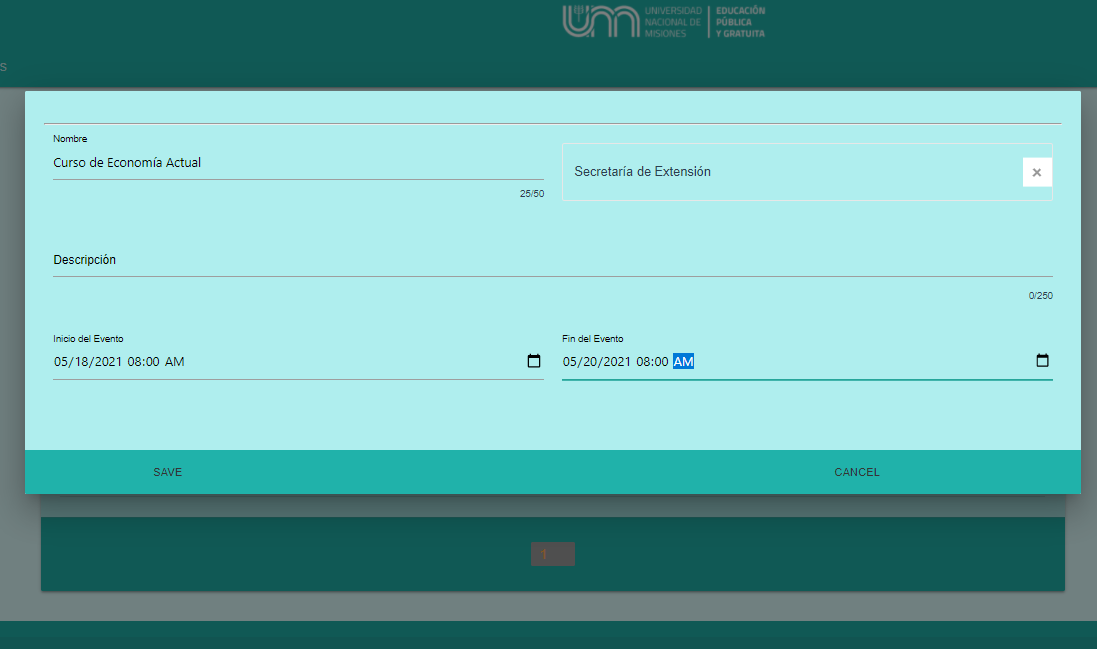
\includegraphics[scale=0.4]{nuevo_evento.png}}
  \caption{Creación de nueva área en el sistema,  Fuente: captura de pantalla. }
  \label{img:nuevo_evento}
\end{figure}




\subsection{Validación de documento}

Finalizado el sistema se probará en un flujo habitual de la Secretaría de Extensión de la \glsfirst{fce}, 
siguiendo los circuitos normales de una actividad realizada por esta área, en base a la información recaudada en la entrevistas realizadas\cite[]{larraburu_secretariextension_2020},
Omitiendo las partes iniciales , comenzando el flujo desde el momento que se crea un documento digital para entregar 
al participante de una actividad.

Los pasos previos antes de  enviar o entregar el documento digital al participante son: 
\begin{enumerate}
  \item Para  sellar el documento en la Blockchain, en la vista “ encontrar documento ” , con la Metamask tener la cuenta del 
  propietario del área activada.
  \item Seleccionar el Área de “ Secretaría de Extensión ” y el Evento “ Curso de Economía Actual ”, el resto de los input se deja vacío.
  \item Luego se da click al botón “ DOCUMENTOS ” y se selecciona los documentos para  generar el hash y almacenarlo en la Blockchain, en el ejemplo de la figura \ref{img:nuevos_certificados} se muestran 3 certificados seleccionados
  que aun no están verificados porque no se encuentran almacenados, se puede observar que el hash de cada uno es diferente, los certificados subidos 
  se pueden ver en el anexo \ref{as:imagenes_pruebas}.
  \begin{figure}[H]
    \centering
    {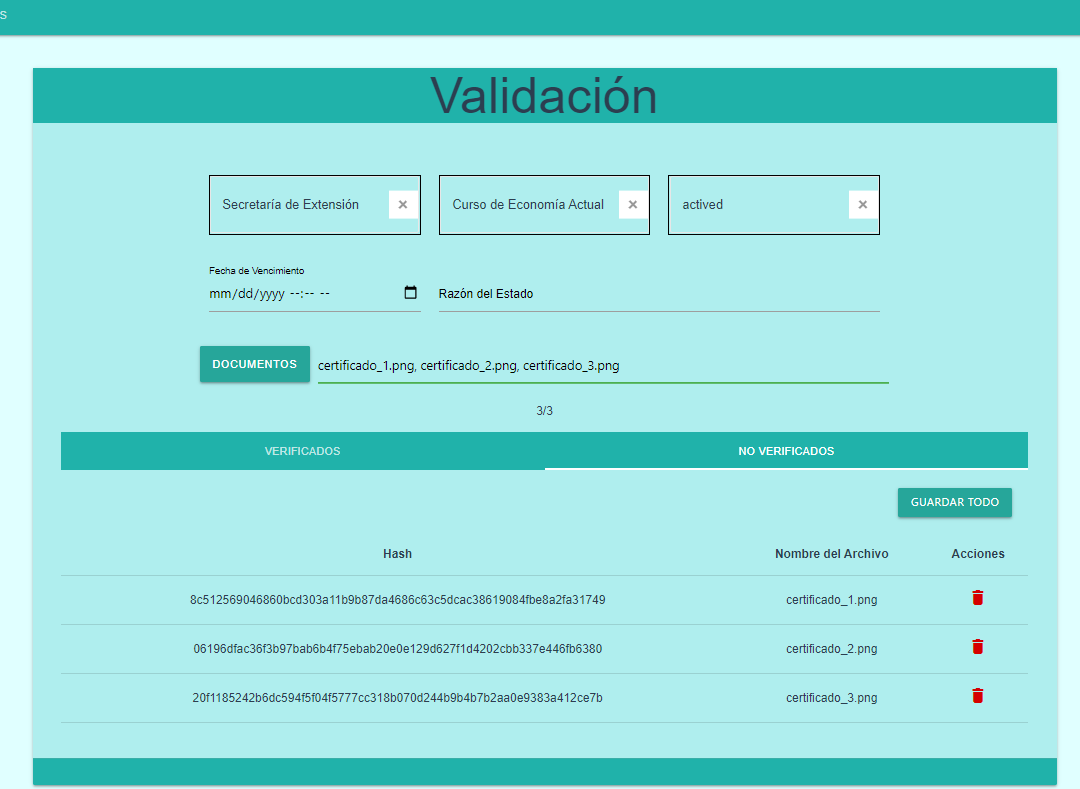
\includegraphics[scale=0.5]{prueba_cargando_certificados.png}}
    \caption{Carga de nuevos documentos,  Fuente: captura de pantalla. }
    \label{img:nuevos_certificados}
  \end{figure}
  \item  El siguiente paso es dar click en el botón “ GUARDAR TODO ”, esto almacena los datos cargados en la Blockchain.
  \item Una vez completada la transacción en la  Blockchain de prueba, los documentos aparecen como verificados ver figura \ref{img:prueba_almacenamiento}.
  \item \begin{figure}[H]
    \centering
    {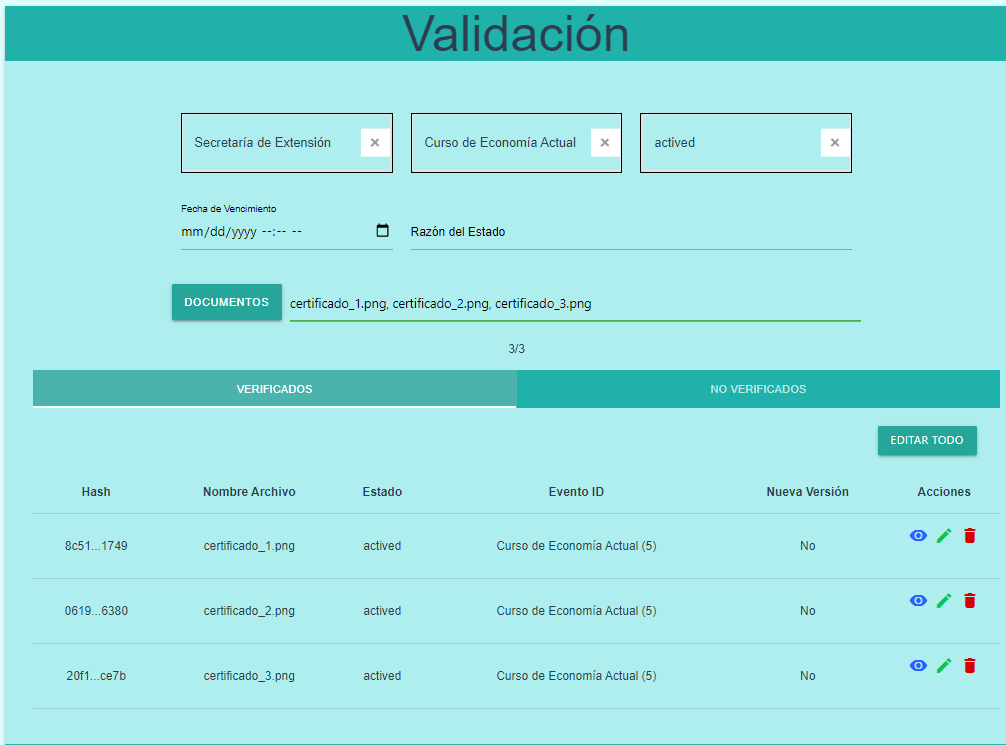
\includegraphics[scale=0.5]{prueba_documento_almacenado.png}}
    \caption{Hash de documentos almacenados y verificados,  Fuente: captura de pantalla. }
    \label{img:prueba_almacenamiento}
  \end{figure}
  \item Cambiando de cuenta y probando el documento  “ certificado\_1 ”, para obtener los resultados. 
\end{enumerate}




Son pocos los pasos necesarios para almacenar los datos en la Blockchain
Para estos pasos se toman en cuentan pre-requisitos, siendo estos, 
la carga previa del área que organiza el evento, con los propietarios del área, 
el evento que emitirá los documentos digitales. 